\documentclass[12pt, letterpaper]{article}
  \usepackage{graphicx}
  \usepackage{pdfpages}
  \usepackage[blocks]{authblk}% The option is for block layout
  \usepackage[pdfborder={0 0 0}]{hyperref}% For email addresses

\title{Analysis of Relationship between PSA and Clinical Measurements}

\author{\textbf{Yujun Chen}}
\affil{\textbf{\url{yjnchen@ucdavis.edu}}}

\author{Siqi Lu}
\affil{\url{sqlu@ucdavis.edu}}

\author{Zhen Zhang}
\affil{\url{ezzhang@ucdavis.edu}}

\begin{document}

  \maketitle

  \newpage

\begin{abstract}

  This paper aims to unravel the relationship between serum $prostate-specific$ $antigen~level$ ($PSA$) and a number of prognostic clinical measurements in men with advanced prostate cancer by building a general linear model on the data observed on 97 men who were about to undergo radical prostatectomies. After model selection, model diagnosis and cross-validation, a model with $cancer~volume$, $weight$, $age$, $benign~prostatic~hyperplasia$, $seminal~vesicle~invasion$ and $Gleason~score$ is chosen. The predictor $capsular$ $penetration$ is proved to be redundant in this model. The relationship between response variable and each predictor is first-order and linear, and is positive except for $age$. The relationship between $PSA$ and $cancer~volume$, $weight$, $seminal~vesicle~invasion$ is highly significant ($p < 0.03$), that between $PSA$ and $age$ and $benign~prostatic~hyperplasia$ is somewhat significant ($p \approx 0.15$). The $Gleason~score~7$ has the same effect as $6$ on $PSA$ ($p = 0.43$), while $8$ has a significantly distinct effect on $PSA$ compared with $6$ ($p = 0.02$). The total coefficient of determination ($R^{2}$) of this model is 0.6385.

\end{abstract}

\newpage
  
\section{Introduction}
  Serum $prostate-specific$ $antigen~level$ ($PSA$) is a useful index in the diagnosis of prostate cancer and the follow-up observations of the patients who underwent radical prostatectomies. Analysis on the relationship between $PSA$ and several prognostic clinical measurements may simplify the process to diagnose the occurrence and reoccurrence of  prostate cancer and thus is a meaningful research. Previous research given by Thomas A. Stamey shows that $PSA$ has a significant relationship with $Gleason~score~7$ or greater, $capsular~penetration$ greater than 1 cm in linear extent, $seminal$ $vesicle~invasion$ and $volume~of~prostate~cancer$\cite{Stamey{1989}}. The following analysis aims to answer these questions: which prediction clinical measurements have effects on the response variable? The relationship is linear or curvilinear? Which predictors have positive effects and which have negative effects? Have we missed some important prediction variables? Does the model suffice? The data used in the analysis was collected on 97 men who were about to undergo radical prostatectomies, for each observation, $patient~ID$, $PSA~level(mb/ml)$, $cancer~volume(cc)$, $weight(gm)$, $age(years)$, $benign$ $prostatic~hyperplasia(cm^{2})$, $seminal~vesicle~invasion$, $capsular$ $penetration(cm)$ and $Gleason score$ were measured and recorded.


\section{Methods and Results}

  \subsection{Data Exploration}

    First we read the data into R, we want to decide the type of each variable, namely distinguish between the quantitative and qualitative variables, so we draw the scatterplot (Figure 1):\\

    From the scatterplot, we found that $PSA$, $cancer~volume$, $weight$, $age$, $benign~prostate~hyperplasia$ and $capsular~penetration$ should be quantitative variables; $seminal~vesicle~invasion$ and $gleason~score$ should be qualitative variables.\\

    Then we analyze the quantitative variables. To get a first sight of the relationship between the quantitative variables, we calculate the correlation matrix between them: From the table, we find that $PSA$ has a moderate relationship with $cancer~volume$ and $capsular~penetration$. We also draw the histogram of these variables (Figure 2). It is seen that $PSA$, $cancer~volume$, $weight$, $age$ and $capsular~penetration$ have a strong pattern of right skewed. We consider doing some transformation, so doing the Box-Cox procedure (Figure 3): It shows a log transformation should be done with the $PSA$ variable. After that, we want to know whether a transformation is needed for the predictors, so we do another scatterplot (Figure 4). From this figure, we find that there is a logarithm pattern between $\log(PSA)$ and $cancer~volume$. So we do a log transformation to $cancer~volume$. In addition, we check whether there is multicollinearity between quantitative variables. Since $VIF$ of each variable is between 1 and 1.7, so there is no indication of high multicollinearity.\\

    For the qualitative variables ($seminal~vesicle~invasion$ and $gleason~score$), we draw a side-by-side boxplot to see whether they have effects on the response variabls (Figure 5): We find that both of them have an impact on $PSA$. Moreover, we draw the interaction boxplot, to see whether the interaction term should be included in this model (Figure 6). We find that there is a mild interaction between them.\\

    Based on these preliminary investigations, we decide:

    \begin{itemize}

      \item to use $\log(PSA)$ as the response variable
      \item to use $log(cancer~volume)$ instead of $cancer~volume$
      \item not to include the interaction term

    \end{itemize}

    Next we should examine whether all predictors are needed, and also whether the first order or the second order should be included in this model.

  \subsection{Model Selection}

    To justify whether a model outperforms other models, we need to test their performance on the validation set. Since we have 97 samples in hand, we randomly split them into a train set with 70 samples, and a test set with 27 samples.

    \subsubsection{First Order Model}

      First we fit the first order model with all predictors. From the output, we find that some of the coefficients are not significant, so we use stepwise procedure to find the best fist order model with different criteria: AIC and BIC, and different direction, forward and backward.\\

      We anticipate four models, but we find that forward and backward select the same model within each criterion. So we result in these two first order models:
      \begin{eqnarray}
        \log(PSA) &=& \beta_0 + \beta_1 * \log(cancer~volume) + \beta_2 * weight + \nonumber\\
                   && \beta_3 * seminal~vesicle~invasion1 + \beta_4 * age + \nonumber\\
                   && \beta_5 * gleason~score7 +\beta_6 * gleason~score8 + \nonumber\\
                   && \beta_7 * benign~prostate~hyperplasia\\
                  &&\nonumber\\
       \log(PSA) &=& \beta_0 + \beta_1 * \log(cancer~volume) + \beta_2 * weight + \nonumber\\
                  && \beta_3 * seminal~vesicle~invasion1 + \beta_4 * age
      \end{eqnarray}

      Model 1 is selected by AIC, and model 2 is selected by BIC. We want to discuss some points here:

      \begin{itemize}

        \item Since BIC puts more penalty on the number of predictors, so BIC tends to select simpler model. Here model 2 is a submodel of model1.
        \item model1 contains $gleason~score$ and $benign~prostate~hyperplasia$, which are not in model2.
        \item We will reserve both these two models, and we want to find whether second order terms can be added into them.

      \end{itemize}

    \subsubsection{Second Order Model}

      First we fit the second order model with all predictors. Since there are so many second order predictors, we need the stepwise procedure to select a subset of them. Again, we use both the AIC and BIC as the criteria, but now we do not start from the null model or full model. For AIC, we start from model 1, while for BIC, we start from model 2. The reason we start from the corresponding first order model is that we want to know whether there is some improvement on the first order model when adding second order terms. The improvement can be a decrease either in AIC or BIC. The models are shown below:
      \begin{eqnarray}
        \log(PSA) &=& \beta_0 + \beta_1 * \log(cancer~volume) + \beta_2 * weight + \beta_3 * age + \nonumber\\
                   && \beta_4 * benign~prostate~hyperplasia * seminal~vesicle~invasion1 + \nonumber\\
                   && \beta_5 * seminal~vesicle~invasion1 + \beta_6 * gleason~score7 + \nonumber\\
                   && \beta_7 * gleason~score8 + \beta_8 * benign~prostate~hyperplasia^2 + \nonumber\\
                   && \beta_9 * benign~prostate~hyperplasia\\
                   &&\nonumber\\
        \log(PSA) &=& \beta_0 + \beta_1 * \log(cancer~volume) + \beta_2 * weight + \nonumber\\
                   && \beta_3 * seminal~vesicle~invasion1 + \beta_4 * age
      \end{eqnarray}

      From above:

      \begin{itemize}

        \item The output suggests model 3 has more predictors than model 1, while model 4 is identical with model 2.
        \item The second order terms have no improvement on BIC criterion.

      \end{itemize}

    \subsubsection{Model Summary}

      Now we have three models in hand. The next step is to do model diagnostic and test them on the validation data to select the best model.

  \subsection{Model Diagnostic and Validation}

    \subsubsection{Model Diagnostic}

      Now we compare the residual vs fitted value plot and qqplot (Figure 7).\\

      From the residual vs fitted value plots, no abnormal pattern is seen. We observe equal spread of residuals along the x axis, which means there is no indication of unequal variance. The relationship is linear.\\

      From the qqplots, that of model 3 shows a slight pattern of heavy tailed. The other two qqplots shows a straight line pattern.\\

      We think that all of these three models pass the model diagnostic, and we will use model validation to select the best one.\\

    \subsubsection{Model Validation}

      To select the best model, we will calculate the MSPE on the test data:

      $$MSPE_v = \frac{\sum^{m}_{j=1}(Y_j - \hat{Y_j})^2}{m}$$

      where $m = 27$, $Y = \log(PSA)$.\\

      The MSPE for model 1 is 2.380, model 2 is 4.996, model 3 is 3.799. We do not compare the fitted coefficients between train and test data within each model, since there are so few samples here, even a good model can have a flexible coefficient. MSPE is much better in this situation.\\

      Model 1 has the smallest MSPE, which means it has the best predict performance. Model 2 has less predictors than model 1, which means that it is underfit, and model 3 has more predictors, which mean it is overfit.\\

      So we choose model 1 as our final model. Next we will fit our final model to the whole data.\\

  \subsection{Final Model Analysis}

    Our final model is:
    \begin{eqnarray}
      \log(PSA) &=& 2.124 + 0.504 * \log(cancer~volume) + 0.002 * weight + \nonumber\\
                 && 0.651 * seminal~vesicle~invasion1  -0.015 * age + \nonumber\\
                 && 0.128 * gleason~score7 + 0.640 * gleason~score8 + \nonumber\\
                 && 0.072 * benign~prostate~hyperplasia
    \end{eqnarray}

    The model summary is shown in the output. And we will plot model diagnostic figures (Figure 8). We find that the 32th case has a very high Cook's distance. So we consider remove it from the model and see whether the results get better.

    The new model coefficient is shown below:
    \begin{eqnarray}
      \log(PSA) &=& 2.042 + 0.489 * \log(cancer~volume) + 0.011 * weight + \nonumber\\
                 && 0.628 * seminal~vesicle~invasion1  -0.017 * age + \nonumber\\
                 && 0.136 * gleason~score7 + 0.574 * gleason~score8 + \nonumber\\
                 && 0.043 * benign~prostate~hyperplasia
    \end{eqnarray}

    We see that the coefficients change a lot, and the adjusted $R^2$ becomes higher, from 0.6221 to 0.6385. In addition, residual standard error decreases from 0.7092 to 0.6967. We also make model diagnostic here (Figure 9), and the results indicate a good fit.\\

    So model 6 is our final result.

\section{Conclusions and Discussion}

  \begin{itemize}

    \item The variables $\log(cancer~volume)$, $weight$, $age$, \textit{benign prostate hyperplasia}, $seminal~vesicle~invasion$ and $gleason~score$ have an effect on the response variable. We do not use $capsular~penetration$.
    \item We derive a linear relationship between predictors and response variables.
    \item All predictors, excluding the $age$ have a positive effect on the response varible, while the $age$ has a negative effect on the reponse variable.
    \item These predictors are adequate since the adjusted $R^2$ is equal to 0.6385.
    \item Our results are general since we fit the model on the train data and test it on the validation data.
    \item The limitation is, it is highly random when we split our data into train and test. Since the size of data is too small, say 97 smaples, the randomness of data will influence our model. The steps to solve this limitation is to either increase the sample size (by bootstrap or have more data), or use cross-validation (LOOCV or 5-fold cross validation) to fit our model.

  \end{itemize}

\begin{thebibliography}{0}
\bibitem{Stamey{1989}}
Stamey, Thomas A., et al. ``Prostate specific antigen in the diagnosis and treatment of adenocarcinoma of the prostate. II. Radical prostatectomy treated patients." The Journal of urology 141.5 (1989): 1076-1083.
\end{thebibliography}

\newpage

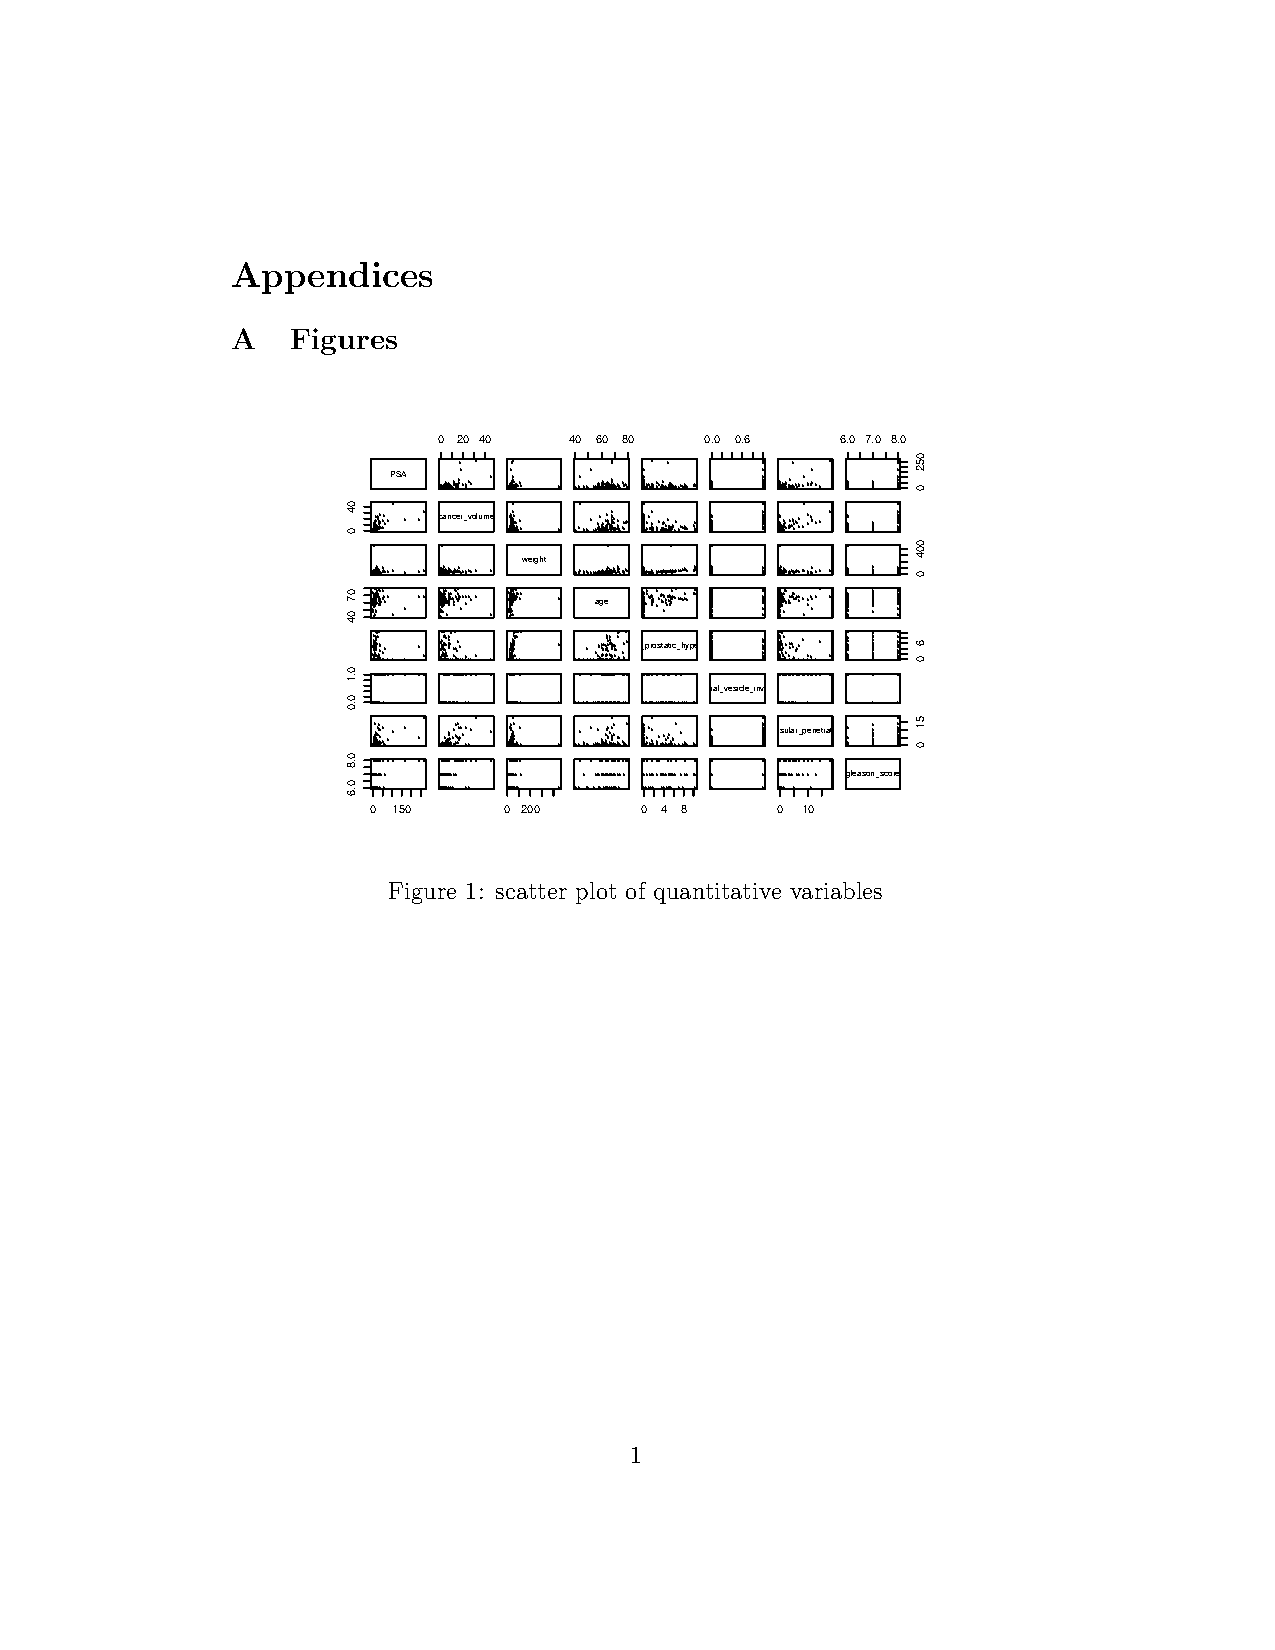
\includepdf[pages = -]{inputs/Figures.pdf}

\newpage

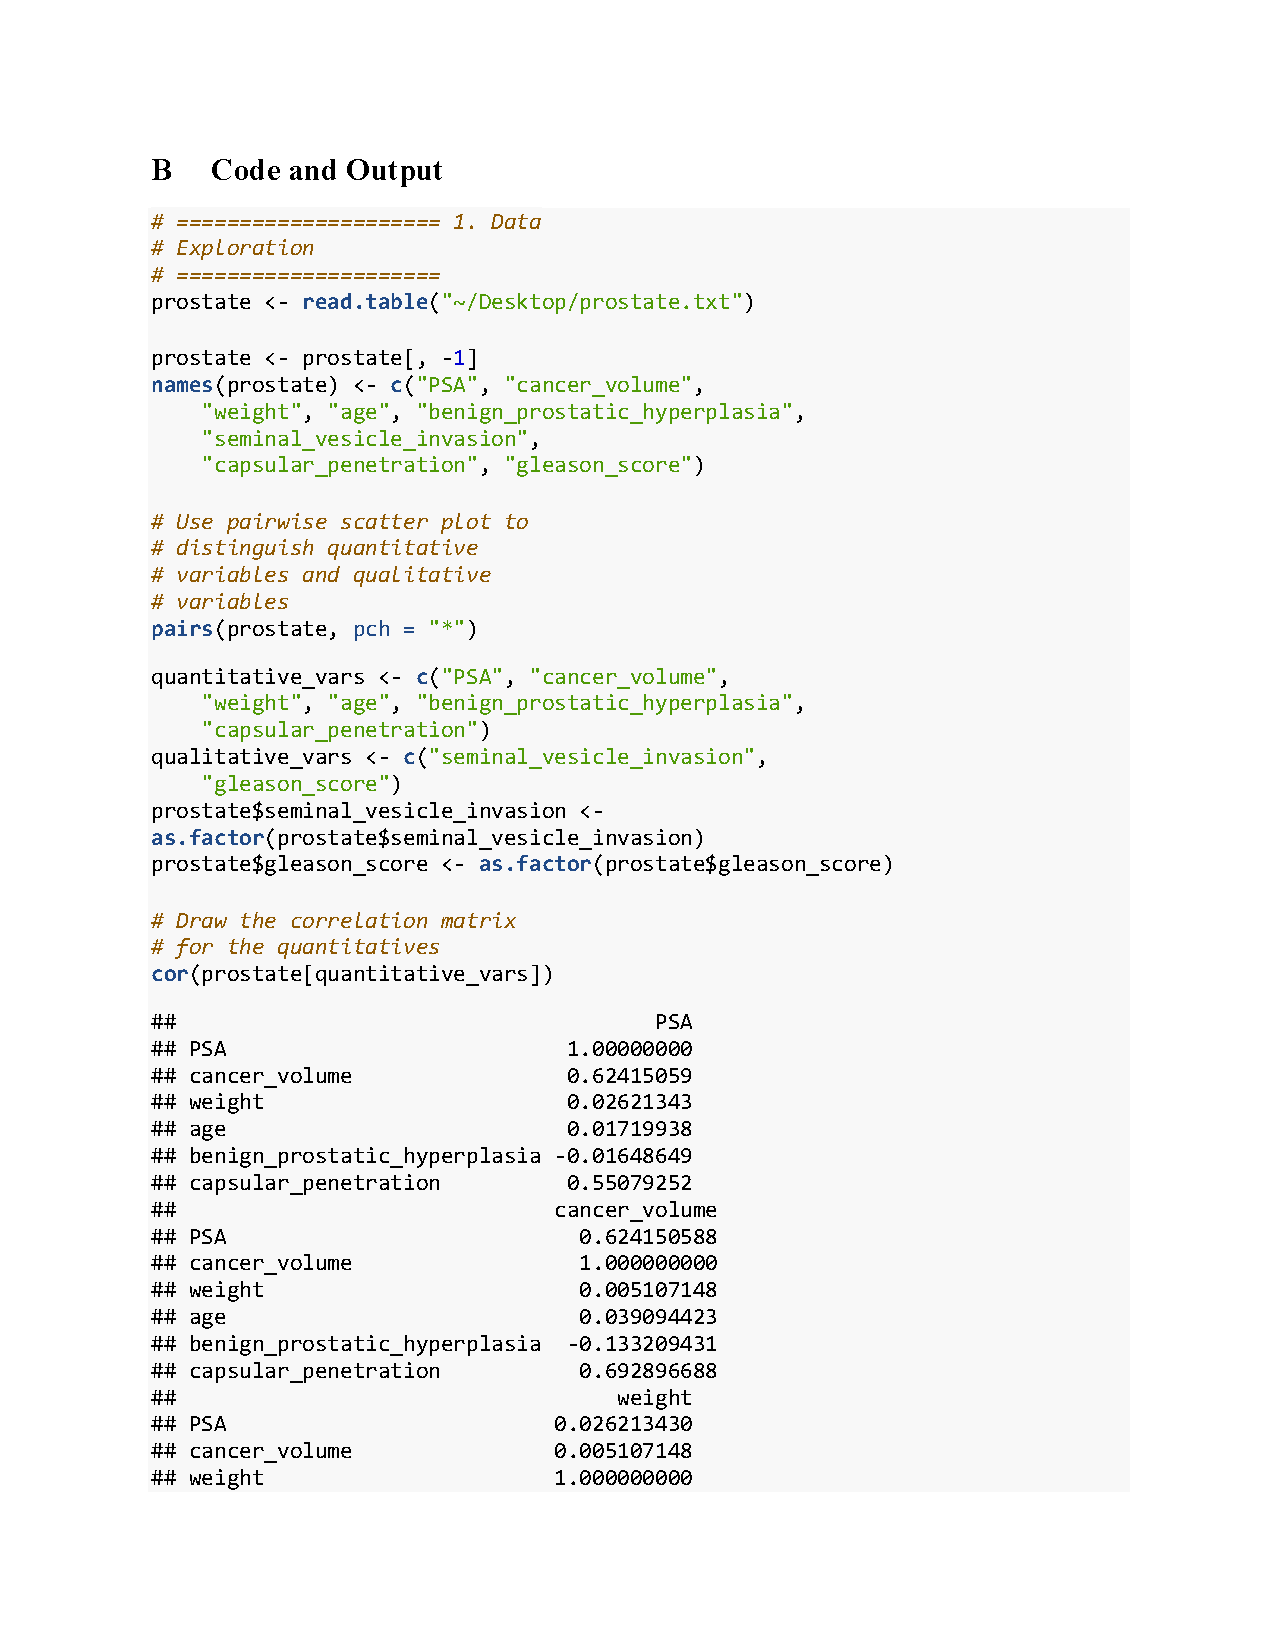
\includepdf[pages=-]{inputs/STA206_codeAndOutput.pdf}

\end{document}
